\documentclass[tikz,border=12pt]{standalone}
\usepackage{amsmath,amssymb}
\usetikzlibrary{positioning,fit,backgrounds,calc,arrows.meta}

\definecolor{foundBg}{HTML}{F7F7F7}\definecolor{foundBorder}{HTML}{555555}
\definecolor{orthBg}{HTML}{E1F5FE}\definecolor{orthBorder}{HTML}{0288D1}
\definecolor{robustBg}{HTML}{E8F5E9}\definecolor{robustBorder}{HTML}{388E3C}
\definecolor{infBg}{HTML}{E8EAF6}\definecolor{infBorder}{HTML}{3949AB}
\definecolor{effBg}{HTML}{FFF3E0}\definecolor{effBorder}{HTML}{F57C00}
\definecolor{higherBg}{HTML}{F3E5F5}\definecolor{higherBorder}{HTML}{7B1FA2}
\definecolor{altBg}{HTML}{E0F2F1}\definecolor{altBorder}{HTML}{00796B}
\definecolor{projBg}{HTML}{FFFDE7}\definecolor{projBorder}{HTML}{F9A825}
\definecolor{limBg}{HTML}{FBE9E7}\definecolor{limBorder}{HTML}{C62828}

\newcommand{\E}{\mathbb{E}}
\newcommand{\src}[1]{\\[1pt]{\scriptsize\color{black!65}#1}}

\begin{document}
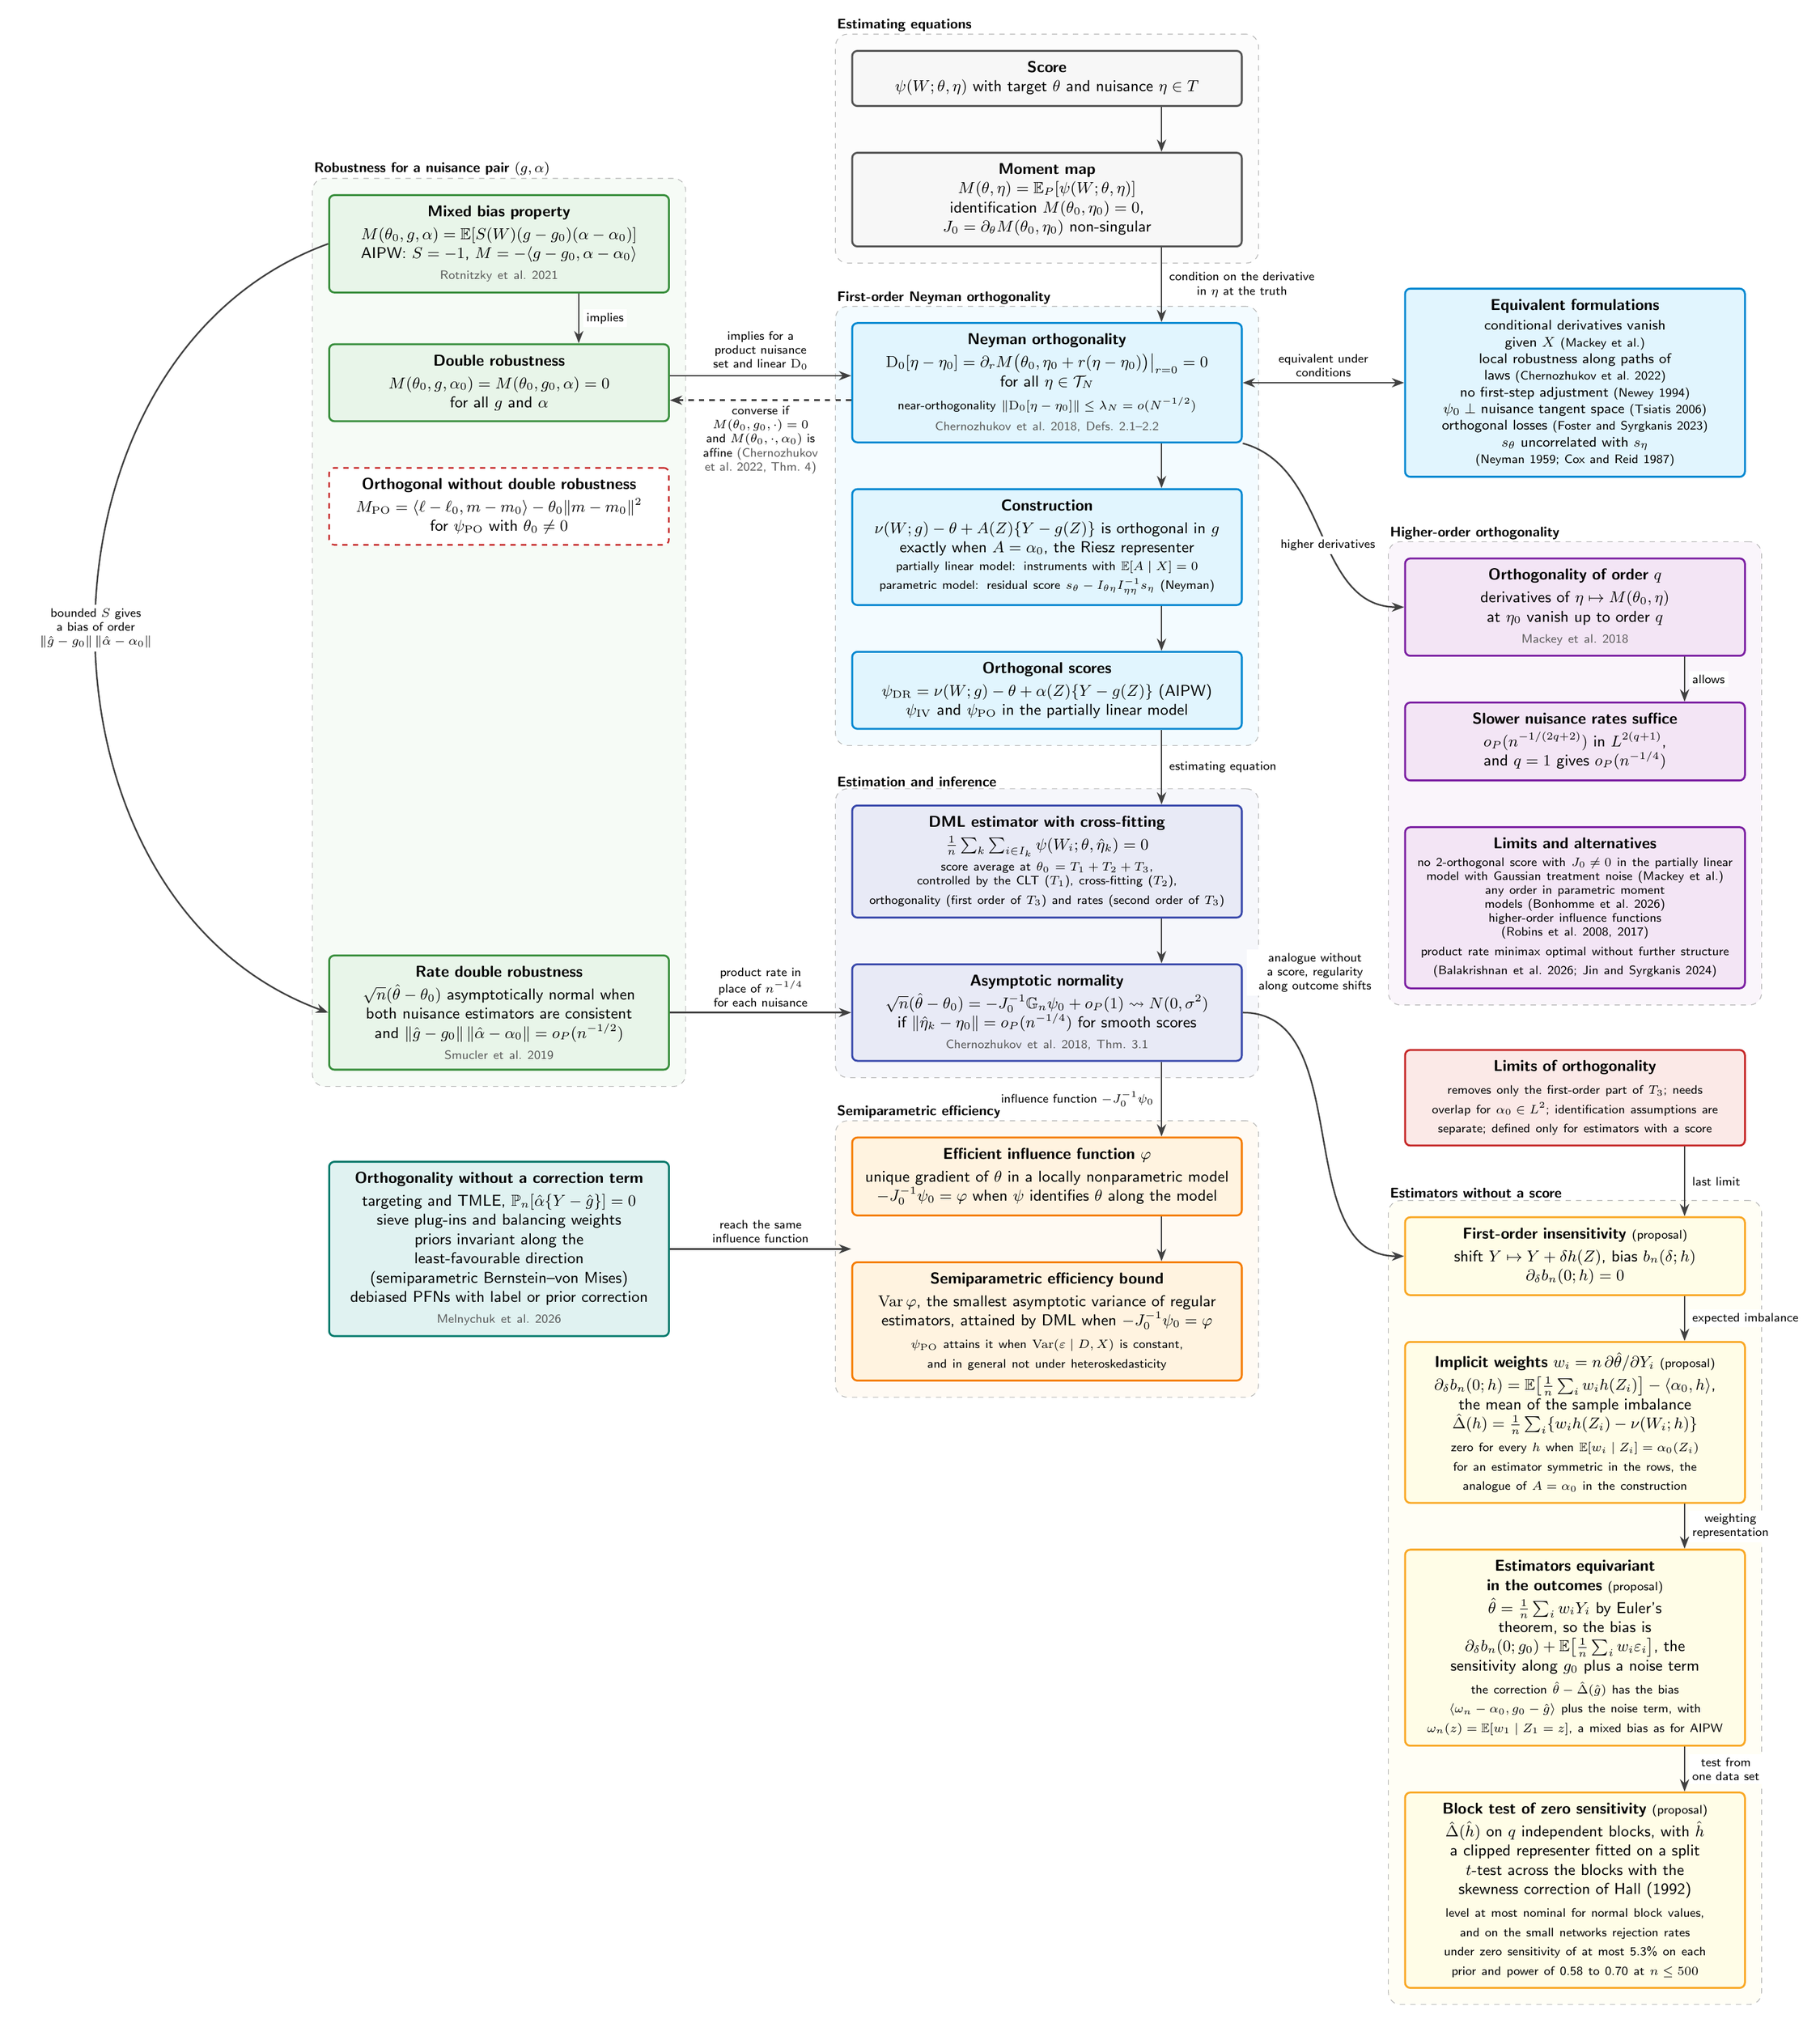
\begin{tikzpicture}[
    >=Stealth,
    font=\small\sffamily,
    every node/.append style={execute at begin node={\thickmuskip=5mu\medmuskip=4mu\thinmuskip=3mu\hyphenpenalty=10000\exhyphenpenalty=10000}},
    box/.style={rectangle, rounded corners=3pt, align=center, inner sep=6pt, text width=#1, draw, line width=1.1pt, text=black},
    box/.default=7.4cm,
    foundation/.style={box, fill=foundBg, draw=foundBorder},
    orth/.style={box, fill=orthBg, draw=orthBorder},
    robust/.style={box=6.4cm, fill=robustBg, draw=robustBorder},
    inf/.style={box, fill=infBg, draw=infBorder},
    eff/.style={box, fill=effBg, draw=effBorder},
    higher/.style={box=6.4cm, fill=higherBg, draw=higherBorder},
    alt/.style={box=6.4cm, fill=altBg, draw=altBorder},
    proj/.style={box=6.4cm, fill=projBg, draw=projBorder},
    lim/.style={box=6.4cm, fill=limBg, draw=limBorder},
    note/.style={box=6.4cm, fill=white, draw=limBorder, dashed, line width=0.9pt},
    edge/.style={->, line width=0.9pt, black!75},
    lbl/.style={fill=white, font=\scriptsize\sffamily, align=center, inner sep=2pt, text=black},
    groupBox/.style={draw=black!30, dashed, rounded corners=7pt, inner sep=9pt},
    head/.style={font=\bfseries\footnotesize\sffamily, text=black, anchor=south west, inner sep=1pt},
]
\coordinate (L) at (-11.0,0);
\coordinate (R) at (10.6,0);

% ---------------- centre column ----------------
\node[foundation] (SF) {\textbf{Score}\\ $\psi(W;\theta,\eta)$ with target $\theta$ and nuisance $\eta\in T$};
\node[foundation, below=0.9cm of SF] (MM) {\textbf{Moment map}\\ $M(\theta,\eta)=\E_P[\psi(W;\theta,\eta)]$\\ identification $M(\theta_0,\eta_0)=0$, $J_0=\partial_\theta M(\theta_0,\eta_0)$ non-singular};
\node[orth, below=1.5cm of MM] (NO) {\textbf{Neyman orthogonality}\\[2pt] $\mathrm D_0[\eta-\eta_0]=\partial_r M\big(\theta_0,\eta_0+r(\eta-\eta_0)\big)\big|_{r=0}=0$\\ for all $\eta\in\mathcal T_N$\\[2pt] {\scriptsize near-orthogonality $\|\mathrm D_0[\eta-\eta_0]\|\le\lambda_N=o(N^{-1/2})$}\src{Chernozhukov et al.\ 2018, Defs.~2.1--2.2}};
\node[orth, below=0.9cm of NO] (CON) {\textbf{Construction}\\[2pt] $\nu(W;g)-\theta+A(Z)\{Y-g(Z)\}$ is orthogonal in $g$\\ exactly when $A=\alpha_0$, the Riesz representer\\[2pt] {\scriptsize partially linear model: instruments with $\E[A\mid X]=0$\\ parametric model: residual score $s_\theta-I_{\theta\eta}I_{\eta\eta}^{-1}s_\eta$ (Neyman)}};
\node[orth, below=0.9cm of CON] (OS) {\textbf{Orthogonal scores}\\[2pt] $\psi_{\mathrm{DR}}=\nu(W;g)-\theta+\alpha(Z)\{Y-g(Z)\}$ (AIPW)\\ $\psi_{\mathrm{IV}}$ and $\psi_{\mathrm{PO}}$ in the partially linear model};
\node[inf, below=1.5cm of OS] (DML) {\textbf{DML estimator with cross-fitting}\\[2pt] $\tfrac1n\sum_k\sum_{i\in I_k}\psi(W_i;\theta,\hat\eta_k)=0$\\[2pt] {\scriptsize score average at $\theta_0$ $=T_1+T_2+T_3$, controlled by the CLT ($T_1$), cross-fitting ($T_2$),\\ orthogonality (first order of $T_3$) and rates (second order of $T_3$)}};
\node[inf, below=0.9cm of DML] (AN) {\textbf{Asymptotic normality}\\[2pt] $\sqrt n(\hat\theta-\theta_0)=-J_0^{-1}\mathbb G_n\psi_0+o_P(1)\rightsquigarrow N(0,\sigma^2)$\\ if $\|\hat\eta_k-\eta_0\|=o_P(n^{-1/4})$ for smooth scores\src{Chernozhukov et al.\ 2018, Thm.~3.1}};
\node[eff, below=1.5cm of AN] (EIF) {\textbf{Efficient influence function} $\varphi$\\[2pt] unique gradient of $\theta$ in a locally nonparametric model\\ $-J_0^{-1}\psi_0=\varphi$ when $\psi$ identifies $\theta$ along the model};
\node[eff, below=0.9cm of EIF] (EB) {\textbf{Semiparametric efficiency bound}\\[2pt] $\operatorname{Var}\varphi$, the smallest asymptotic variance of regular estimators, attained by DML when $-J_0^{-1}\psi_0=\varphi$\\[2pt] {\scriptsize $\psi_{\mathrm{PO}}$ attains it when $\operatorname{Var}(\varepsilon\mid D,X)$ is constant, and in general not under heteroskedasticity}};

% ---------------- left column ----------------
\node[robust, anchor=center] (DR) at (NO -| L) {\textbf{Double robustness}\\[2pt] $M(\theta_0,g,\alpha_0)=M(\theta_0,g_0,\alpha)=0$\\ for all $g$ and $\alpha$};
\node[robust, above=1.0cm of DR] (MBP) {\textbf{Mixed bias property}\\[2pt] $M(\theta_0,g,\alpha)=\E[S(W)(g-g_0)(\alpha-\alpha_0)]$\\ AIPW: $S=-1$, $M=-\langle g-g_0,\alpha-\alpha_0\rangle$\src{Rotnitzky et al.\ 2021}};
\node[note, below=0.9cm of DR] (CE) {\textbf{Orthogonal without double robustness}\\[2pt] $M_{\mathrm{PO}}=\langle\ell-\ell_0,m-m_0\rangle-\theta_0\|m-m_0\|^2$\\ for $\psi_{\mathrm{PO}}$ with $\theta_0\neq0$};
\node[robust, anchor=center] (RDR) at (AN -| L) {\textbf{Rate double robustness}\\[2pt] $\sqrt n(\hat\theta-\theta_0)$ asymptotically normal when both nuisance estimators are consistent and $\|\hat g-g_0\|\,\|\hat\alpha-\alpha_0\|=o_P(n^{-1/2})$\src{Smucler et al.\ 2019}};
\coordinate (effmid) at ($(EIF)!0.5!(EB)$);
\node[alt, anchor=center] (ALT) at (effmid -| L) {\textbf{Orthogonality without a correction term}\\[2pt] targeting and TMLE, $\mathbb P_n[\hat\alpha\{Y-\hat g\}]=0$\\ sieve plug-ins and balancing weights\\ priors invariant along the least-favourable direction (semiparametric Bernstein--von Mises)\\ debiased PFNs with label or prior correction\src{Melnychuk et al.\ 2026}};

% ---------------- right column ----------------
\node[orth, box=6.4cm, anchor=center, font=\footnotesize\sffamily] (FORM) at (NO -| R) {\textbf{\small Equivalent formulations}\\[2pt]
  conditional derivatives vanish given $X$ {\scriptsize(Mackey et al.)}\\
  local robustness along paths of laws {\scriptsize(Chernozhukov et al.\ 2022)}\\
  no first-step adjustment {\scriptsize(Newey 1994)}\\
  $\psi_0\perp$ nuisance tangent space {\scriptsize(Tsiatis 2006)}\\
  orthogonal losses {\scriptsize(Foster and Syrgkanis 2023)}\\
  $s_\theta$ uncorrelated with $s_\eta$ {\scriptsize(Neyman 1959; Cox and Reid 1987)}};
\node[higher, below=1.6cm of FORM] (HOO) {\textbf{Orthogonality of order $q$}\\[2pt] derivatives of $\eta\mapsto M(\theta_0,\eta)$ at $\eta_0$ vanish up to order $q$\src{Mackey et al.\ 2018}};
\node[higher, below=0.9cm of HOO] (RATES) {\textbf{Slower nuisance rates suffice}\\[2pt] $o_P(n^{-1/(2q+2)})$ in $L^{2(q+1)}$, and $q=1$ gives $o_P(n^{-1/4})$};
\node[higher, below=0.9cm of RATES] (HLIM) {\textbf{Limits and alternatives}\\[2pt] {\scriptsize no 2-orthogonal score with $J_0\neq0$ in the partially linear model with Gaussian treatment noise (Mackey et al.)\\ any order in parametric moment models (Bonhomme et al.\ 2026)\\ higher-order influence functions (Robins et al.\ 2008, 2017)\\ product rate minimax optimal without further structure (Balakrishnan et al.\ 2026; Jin and Syrgkanis 2024)}};
\node[lim, below=1.2cm of HLIM] (LIM) {\textbf{Limits of orthogonality}\\[2pt] {\scriptsize removes only the first-order part of $T_3$; needs overlap for $\alpha_0\in L^2$; identification assumptions are separate; defined only for estimators with a score}};
\node[proj, below=1.4cm of LIM] (FOI) {\textbf{First-order insensitivity} {\scriptsize(proposal)}\\[2pt] shift $Y\mapsto Y+\delta h(Z)$, bias $b_n(\delta;h)$\\ $\partial_\delta b_n(0;h)=0$};
\node[proj, below=0.9cm of FOI] (IW) {\textbf{Implicit weights} $w_i=n\,\partial\hat\theta/\partial Y_i$ {\scriptsize(proposal)}\\[2pt] $\partial_\delta b_n(0;h)=\E\big[\tfrac1n\sum_iw_ih(Z_i)\big]-\langle\alpha_0,h\rangle$, the mean of the sample imbalance $\hat\Delta(h)=\tfrac1n\sum_i\{w_ih(Z_i)-\nu(W_i;h)\}$\\[2pt] {\scriptsize zero for every $h$ when $\E[w_i\mid Z_i]=\alpha_0(Z_i)$ for an estimator symmetric in the rows, the analogue of $A=\alpha_0$ in the construction}};
\node[proj, below=0.9cm of IW] (EQ) {\textbf{Estimators equivariant in the outcomes} {\scriptsize(proposal)}\\[2pt] $\hat\theta=\tfrac1n\sum_iw_iY_i$ by Euler's theorem, so the bias is\\ $\partial_\delta b_n(0;g_0)+\E\big[\tfrac1n\sum_iw_i\varepsilon_i\big]$, the sensitivity along $g_0$ plus a noise term\\[2pt] {\scriptsize the correction $\hat\theta-\hat\Delta(\hat g)$ has the bias $\langle\omega_n-\alpha_0,g_0-\hat g\rangle$ plus the noise term, with $\omega_n(z)=\E[w_1\mid Z_1=z]$, a mixed bias as for AIPW}};
\node[proj, below=0.9cm of EQ] (BT) {\textbf{Block test of zero sensitivity} {\scriptsize(proposal)}\\[2pt] $\hat\Delta(\hat h)$ on $q$ independent blocks, with $\hat h$ a clipped representer fitted on a split\\ $t$-test across the blocks with the skewness correction of Hall (1992)\\[2pt] {\scriptsize level at most nominal for normal block values, and on the small networks rejection rates under zero sensitivity of at most 5.3\% on each prior and power of 0.58 to 0.70 at $n\le500$}};

% ---------------- group boxes ----------------
\begin{scope}[on background layer]
  \node[groupBox, fill=foundBg!40, fit=(SF)(MM)] (g1) {};
  \node[groupBox, fill=orthBg!40, fit=(NO)(CON)(OS)] (g2) {};
  \node[groupBox, fill=infBg!40, fit=(DML)(AN)] (g3) {};
  \node[groupBox, fill=effBg!40, fit=(EIF)(EB)] (g4) {};
  \node[groupBox, fill=robustBg!40, fit=(MBP)(DR)(CE)(RDR)] (g5) {};
  \node[groupBox, fill=higherBg!40, fit=(HOO)(RATES)(HLIM)] (g6) {};
  \node[groupBox, fill=projBg!40, fit=(FOI)(IW)(EQ)(BT)] (g7) {};
\end{scope}
\node[head] at (g1.north west) {Estimating equations};
\node[head] at (g2.north west) {First-order Neyman orthogonality};
\node[head] at (g3.north west) {Estimation and inference};
\node[head] at (g4.north west) {Semiparametric efficiency};
\node[head] at (g5.north west) {Robustness for a nuisance pair $(g,\alpha)$};
\node[head] at (g6.north west) {Higher-order orthogonality};
\node[head] at (g7.north west) {Estimators without a score};

% ---------------- edges ----------------
\def\off{2.3cm}
\draw[edge] ([xshift=\off]SF.south) -- ([xshift=\off]MM.north);
\draw[edge] ([xshift=\off]MM.south) -- node[lbl, right=2pt] {condition on the derivative\\ in $\eta$ at the truth} ([xshift=\off]NO.north);
\draw[edge] ([xshift=\off]NO.south) -- ([xshift=\off]CON.north);
\draw[edge] ([xshift=\off]CON.south) -- ([xshift=\off]OS.north);
\draw[edge] ([xshift=\off]OS.south) -- node[lbl, right=2pt] {estimating equation} ([xshift=\off]DML.north);
\draw[edge] ([xshift=\off]DML.south) -- ([xshift=\off]AN.north);
\draw[edge] ([xshift=\off]AN.south) -- node[lbl, left=2pt] {influence function $-J_0^{-1}\psi_0$} ([xshift=\off]EIF.north);
\draw[edge] ([xshift=\off]EIF.south) -- ([xshift=\off]EB.north);

\draw[edge] ([xshift=1.6cm]MBP.south) -- node[lbl, right=2pt] {implies} ([xshift=1.6cm]DR.north);
\draw[edge] ([yshift=4pt]DR.east) -- node[lbl, above=1pt, text width=2.6cm] {implies for a product nuisance set and linear $\mathrm D_0$} ([yshift=4pt]NO.west |- DR.east);
\draw[edge, dashed] ([yshift=-10pt]NO.west |- DR.east) -- node[lbl, below=1pt, text width=2.6cm] {converse if $M(\theta_0,g_0,\cdot)=0$ and $M(\theta_0,\cdot,\alpha_0)$ is affine {\color{black!65}(Chernozhukov et al.\ 2022, Thm.~4)}} ([yshift=-10pt]DR.east);
\draw[edge] (MBP.west) to[out=200, in=160, looseness=1.1] node[lbl, pos=0.5, align=center] {bounded $S$ gives\\ a bias of order\\ $\|\hat g-g_0\|\,\|\hat\alpha-\alpha_0\|$} (RDR.west);
\draw[edge] (RDR) -- node[lbl, above=1pt, text width=2.6cm] {product rate in place of $n^{-1/4}$ for each nuisance} (AN);
\draw[edge] (ALT.east) -- node[lbl, above=1pt, text width=2.4cm] {reach the same influence function} (ALT.east -| EIF.west);

\draw[edge, <->] (NO.east |- FORM) -- node[lbl, above=1pt, text width=2.4cm] {equivalent under conditions} (FORM.west);
\draw[edge] (NO.south east) to[out=-15, in=180] node[lbl, pos=0.55, text width=2.0cm] {higher derivatives} (HOO.west);
\draw[edge] ([xshift=2.2cm]HOO.south) -- node[lbl, right=2pt] {allows} ([xshift=2.2cm]RATES.north);
\draw[edge] (AN.east) to[out=0, in=180] (FOI.west);
\node[lbl, text width=2.6cm] at ($(AN.east)+(1.45,0.8)$) {analogue without a score, regularity along outcome shifts};
\draw[edge] ([xshift=2.2cm]LIM.south) -- node[lbl, right=2pt] {last limit} ([xshift=2.2cm]FOI.north);
\draw[edge] ([xshift=2.2cm]FOI.south) -- node[lbl, right=2pt] {expected imbalance} ([xshift=2.2cm]IW.north);
\draw[edge] ([xshift=2.2cm]IW.south) -- node[lbl, right=2pt] {weighting\\ representation} ([xshift=2.2cm]EQ.north);
\draw[edge] ([xshift=2.2cm]EQ.south) -- node[lbl, right=2pt] {test from\\ one data set} ([xshift=2.2cm]BT.north);
\end{tikzpicture}
\end{document}
